\documentclass{article}
\usepackage[utf8]{inputenc}

\title{Chem-131C-Lec9}

\author{swflynn }
\date{April 2017}

\usepackage{natbib}
\usepackage{graphicx}
\usepackage{braket}
\usepackage{amsmath}
\usepackage[margin=0.7in]{geometry}
\usepackage{subfigure}

\begin{document}

\maketitle

\section*{Lecture 9; 4/21/17}
We have alluded to entropy being related to probability, in this lecture we are going to investigate some probability theory. 
Consider flipping a coin, this system has 2 states (S=2) and there are M coins. 
This is a binomial (binary system) so lets call the heads result 0 and the tails 1. 
If we have a coin it will have probabilities of (1-a) and a for the two different faces (notice these sum to 1 which is required for a probability distribution). 
If the coin is fair then a=0.5, and we would write
\begin{equation}
    P_0 = \frac{1}{2} \qquad P_1 = \frac{1}{2}
\end{equation}
Lets now flip 2 coins (m=2, s=2), we can count all the possible results; 00, 01, 10, and 11. 
Because the coin flips are \textbf{Independent} we simply multiply the probabilities. 
\begin{equation}
\begin{split}
    P(0,0) &= \frac{1}{4} \qquad P(0,1) = \frac{1}{4} \qquad P(1,0) = \frac{1}{4} \qquad P(1,1) = \frac{1}{4} \\
    P_0 &= \frac{1}{4} \qquad P_1 = \frac{1}{2}  \qquad P_2 = \frac{1}{4}
    \end{split}
\end{equation}
The notation on the first line simply gives heads or tails to the coordinates, the second line lists the number of heads that occur in an event. 
The number of heads can be thought of as a collective variable (we are grouping more information into a single variable) and is very useful in more complicated probability questions. 

As a side note, the coin flipping probabilities being multiplied is not a general phenomenon. 
The coins do not know or care what any other coin lands on, it simply will not effect their individual coin toss. 
The coin also does not care what its previous coin toss result was, the coin has no 'history' of the events. 
In these specific circumstances are true than you can simply multiply the probabilities of consecutive events as we do with coin flipping. 

If we want to flip 3 coins we can again simply calculate all the states, or we can realize that this event is a binomial, and the number of states in a binomial is given by 
\begin{equation}
S^M
\end{equation}
Therefore 3 coin flips will have $2^3$ = 8 combinations. 
The combinations are (0,0,0) (1,0,0) (0,1,0) (0,0,1) (1,1,0) (1,0,1) (0,1,1) and (1,1,1). 
We can write the collective variable as the number of heads and we find. 
\begin{equation}
P_0 = \frac{1}{8} \qquad P_1 = \frac{3}{8} \qquad P_2=\frac{3}{8} \qquad P_3=\frac{1}{8}
\end{equation}

As stated above this is a binomial system, the binomial is introduced in various ways, most commonly as n choose k. 
\begin{equation}
\binom{n}{k} \equiv \frac{n!}{k! (n-k)!}
\end{equation}
This equation is used to find how to get k 'things' out of n total 'things'. 
It may have appeared in your algebra class, it can be used to calculate the coefficients to a binomial expansion. 
\begin{equation}
(a+b)^2 = a^2 + 2ab+ b^2
\end{equation}
We interpret these coefficients as a probability (un-normalized) so we just add in a normalization factor C. 
\begin{equation}
P_j = C\left(\frac{n}{j} \right)
\end{equation}
In your mathematics class the binomial will be written a bit differently. 
\begin{equation}
(a+b)^n = \sum_{k=0}^N \binom{n}{k}a^kb^{n-k}
\end{equation}
Consider a = b = 1
\begin{equation}
(2)^n = \sum_{k=0}^N \binom{n}{k}
\end{equation}
So we see the normalization for the binomial must be $\frac{1}{2^N}$. 
So we can write a general formula as 
\begin{equation}
P_j = \frac{1}{2^N}\left(\frac{n}{j} \right)
\end{equation}

\subsection*{Multinomial Coefficient}
We can also generalize to higher term polynomials. 
\begin{equation}
(a+b+c)^n = \sum_{k_1}\sum_{k_2}\sum_{k_3}\binom{n}{k_1 k_2 k_3} a^{k_1}b^{k_2}c^{k_3}
\end{equation}
Note here n is the total power ($k_1+k_2+k_3 = n$)
And the binomial can be written as 
\begin{equation}
\binom{n}{k_1 k_2 k_3} = \frac{n!}{k_1!k_2!k_3!}
\end{equation}


\subsection*{Probability Generating Function}
This is yet another example that is not going to be on the final, but is interesting. 
A probability generating function is simply a function that can be used to calculate probabilities, it should be no surprise it uses our good friend derivatives to do it!

For a fair coin it turns out that
\begin{equation}
PGF \equiv F(x) = \frac{1}{2} + \frac{1}{2}x
\end{equation}
The reason PGF are useful is
\begin{equation}
P_i = \frac{1}{i!}\frac{\partial^i}{\partial x^i}[F(x)]
\end{equation}
So the various probabilities are calculated using higher and higher order derivatives. 

In general we can write 
\begin{equation}
F(x) = \sum_{k=0}^n P_kx^k
\end{equation}
Consider 1 and 2 coins we have
\begin{equation}
\begin{split}
    F_1(x) = \frac{1}{2} + \frac{1}{2}x \\
    F_2(x) = F_1^2(x) = \frac{1}{4} + \frac{1}{2}x + \frac{1}{4}x^2
\end{split}
\end{equation}
So this method is preferred for calculating the probabilities of composite event (when you do something a few times and then do something else a few times). 

\subsection*{Rolling Dice}
We will assume we have 6-sided dice and each face has an equal probability of landing face-up.
The probability generating function for the dice is as follows.
\begin{equation}
F_1(x) = \frac{1}{6}[x+x^2+x^3+x^4+x^5+x^6]
\end{equation}
If we now roll 2 separate dice we find 
\begin{equation}
F_1^2(x) = \frac{1}{36}[x^2 + 2x^3 + 3x^4 + 4x^5 + 5x^6 + 6x^7 + 5x^8 + 4x^9 + 3x^{10} + 2x^{11} + x^{12} ]
\end{equation}
Remember this equation tells us there is 1 out of 36 ways to get snake eyes with the 2 rolls, 2 out of 36 ways to get a sum of 3 with the 2 dice, and etc. 
We note that there is no x$^0$ or x$^1$ because we are rolling 2 dice and therefore cannot get a sum less than 2. 

\subsection*{Pachinko}
This game works something like you drop a ball into a grid of posts, and then you watch the trajectory of the ball as it falls through the maze of posts. 
At first thought this game seems pretty easy, each pin we hit has 2 choices, left or right, and ohhhh look a binomial again!
However, if you watch a few trajectories (the time sequence of the ball falling is a trajectory) you start to notice that seemingly the same initial position of the ball can generate a very different final position. 
That is the whole reason this can be used as a gambling game, if it were too easy the player would always win.

This is a good physical representation of \textbf{Chaos Theory}.
This branch of mathematics/dynamics considers systems where a very slight change in the initial conditions of the system propagate to a massively (exponentially) different final result. 
For pachinko, slightly changing the initial position of the ball will lead to a slightly different first collision, which will propagate larger and larger deviations in all the subsequent collisions. 
After even a few events (collisions) there is very little certainty in where the trajectory of the ball will end. 

This is still a binomial, if we consider 6 different collision events we find
\begin{equation}
F_6(x) = (\frac{1}{2} + \frac{1}{2}x)^6 \implies \frac{1}{2^6}\sum_{k=1}^6\binom{6}{k}x^k
\end{equation}
As the normalization factor should tell you, there are a massive number of possibilities after the 6 events. 

In life, if you have a large number of independent events you actually generate a Gaussian Distribution!
Stated a bit differently, when we sum over various independent events (like each collision in Pachinko), you end up generating a normal distribution.
This is known as the \textbf{Central Limit Theorem}. 
So we could actually forget using our binomial distribution to understand Pachinko, and instead use a normal distribution. 

\subsection*{Entropy....Finally}
Entropy should be thought of as the likelihood of some arrangement occurring. 
It is directional, meaning certain events are more likely to occur than others. 
If we have N particles and S states we can start considering arrangements.
Consider 2 dice, N=2 and S=6, these two facts will define our \textbf{Configuration Space}. 
The configuration space is the collection of possible results you can have for a given trial. 
We are interested in the probability of different configurations within this space. 
Consider a role of 3 dice now, we get a 1, 2, and 3 for the faces of the dice. 
We are not sure which dice was which, there are 6 different possibilities for this event (the first dice has 3 choices, then the next dice has 2 choices, and finally 1 choice for the remaining dice = 3!). 

What if we rolled 1,1,2 for the faces? 
The same analysis would make you think there are again 6 different paths. 
But remember we cannot tell the dice apart, this means we are over-counting and will need to divide by a factor. 
\begin{equation}
\frac{6!}{2!1!0!0!0!0!}
\end{equation}
The general equation for this scenario of N particles and S states with potential repetition is
\begin{equation}
W = \frac{N!}{N_1!N_2!\cdots N_S!} = \frac{N!}{\displaystyle \prod_{j=1}^S N_j!}
\end{equation}
This equation is true only for independent equal probability events!
It tells us there are W ways of getting a specific configuration. 

\section{Supplementary Notes}
\subsection{Binomial Review} 
The Binomial family considers n independent trails where each trial has a probability of only 2 events occurring. 
If we call p the probability of success, and 1-p the probability of failure (it is best to pose your binomial questions in this way) than we can write. 
\begin{equation}
    B_{n,p} = \binom{n}{k}p^k(1-p)^{n-k}
\end{equation}
This can be directly connected to the famous Pascal's triangle through induction. 
Take the simple case of n=2
\begin{equation}
\begin{split}
    (a+b)^n &= \sum_{i=0}^n \binom{n}{i}a^{n-i}b^i\\
    (a+b)^2 &= \binom{2}{0}a^{2-0}b^0 + \binom{2}{1}a^{2-1}b^1 + \binom{2}{2}a^{2-2}b^2\\
    (a+b)^2 &= a^2+2ab+b^2
    \end{split}
\end{equation}

\subsection{Probability Generating Function}
A Probability Generating Function (PGF) comes from discrete mathematics. 
If you are interested in running an experiment and counting the number of successful outcomes (flip a few coins, call heads a success) you can write a PGF. 
We write p$_i$ as the probability of getting i successful results per experiment (flip 2 coins, get 1 heads = p$_1$). 
With this type of experiment we can write the PGF in terms of a dummy variable t, which has no meaning, but the power of t tracks the probability we are studying. 
\begin{equation}
    PGF(t) = p_0 + p_1t + p_2t + \cdots p_nt^n
\end{equation}
We note that PGF(1) is our normalization condition, consider the case of rolling 2 dice again. 
\begin{equation}
    PGF(t) = \frac{1}{36}[ t^2 + 2t^3 + 3t^4 + \cdots + 2t^{11} + t^{12}]
\end{equation}
If you now substitute t=1 into the expression you will find g(1) = 1, which is necessary for the function to be a probability. 

\subsection{Chaos Theory}
This is a very deep branch of mathematics/physics that is interested in dynamical systems (time dependent systems), that are very sensitive to the conditions at their origin. 
Although chaotic dynamics and systems are well beyond the scope of any undergraduate course, we can get a feeling for the problem (it turns out these are very difficult problems).
Before quantum mechanics we had Newtonian mechanics, which are innately deterministic. 
This means you put in your values and you always get the same result, there is no probability to consider, there is no 'chance'. 
And as you can assume, this is a good starting model, but it leads to issues when you start diving deep, especially in a quantum mechanical world.
However, we do not need quantum mechanics to start causing problems (yes there is a separate field called quantum chaos). 
Even using deterministic mechanics, if the initial conditions are slightly different you get exponentially different trajectories. 

The land of non-linear differential equations is how you would go about predicting the future of a complicated system, the methods for doing this are... well... good luck. 
A guy named Edward Lorenz (MIT meteorologist) wanted to predicted things like weather, and pioneered the field of chaos theory and coined the term 'the butterfly effect'. 
Essentially he was running simulations, he wanted to re-calculate a trajectory and due to rounding error in  the program he had a slightly different starting point for his calculation. 
This generated a completely different trajectory, and eventually led him to develop the idea of chaotic dynamics. 
It is important to note that each event in a simulation is deterministic, just the slight change in initial conditions causes the divergence. 
Quantum chaos attempts to take into account the effect of probability on the events too, making it even more complicated.
So even though the events in the system are deterministic we are not able to predict them (this could be a problem, uncertainty principle tells us that we are not going to get all the initial conditions very accurately...).

So when you are building a model for a system you are innately assuming and simplifying things to get a deeper understanding of the world. 
You choose specific variables to represent this system, you are able to measure them to some certainty, and all of these assumptions may or may not accurately represent the system!
Clearly when you start discussing these types of topics it is very easy to get lost in philosophical arguments, forget your chemistry degree, grow a beard, and start reading Nietzsche. 

So the moral of the story, if someone asks you how the universe began, you ask them what type of dynamics the universe uses, and hope they are not chaotic or quantum chaotic!


\subsection{Central Limit Theorem}
We are leaving the realm of mathematics and entering the area of statistics (be warned probability theory is mathematics, statistics is science!). 
The central limit theorem comes up all over the place, it is valid for both discrete and continuous distributions. 
As long as your distribution has a well defined mean and variance you can actually generate a normal distribution. 
The way this works, consider rolling a dice (or any experiment) n number of times per trial. 
So you have n data points, and then take their average. 
Meaning roll a dice 4 times, you get values 1, 2, 3, 6 and your average would be 3. 
Now repeat the process, do another 4 trials and calculate the new mean, it will be a different number most likely. 
Now plot the frequency of each mean you generate. 
As you increase the number of trials you run, you will start to approach a normal distribution. 
If we now take a larger number of dice rolls for each trail we will get the same average value, but a much better approximation of a normal distribution. 

\begin{figure}[h!]
\subfigure[Individual Functions]{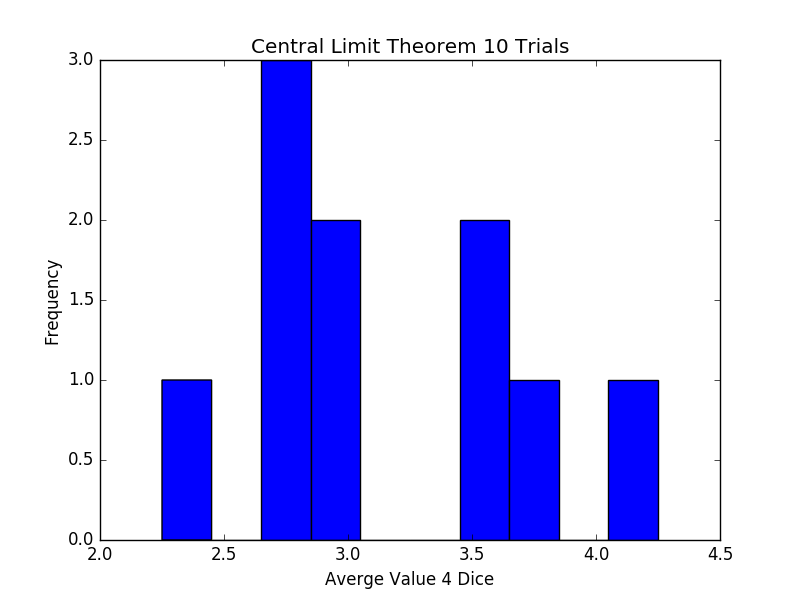
\includegraphics[scale=0.44]{clt10.png}}
\subfigure[Integrand Scaling]{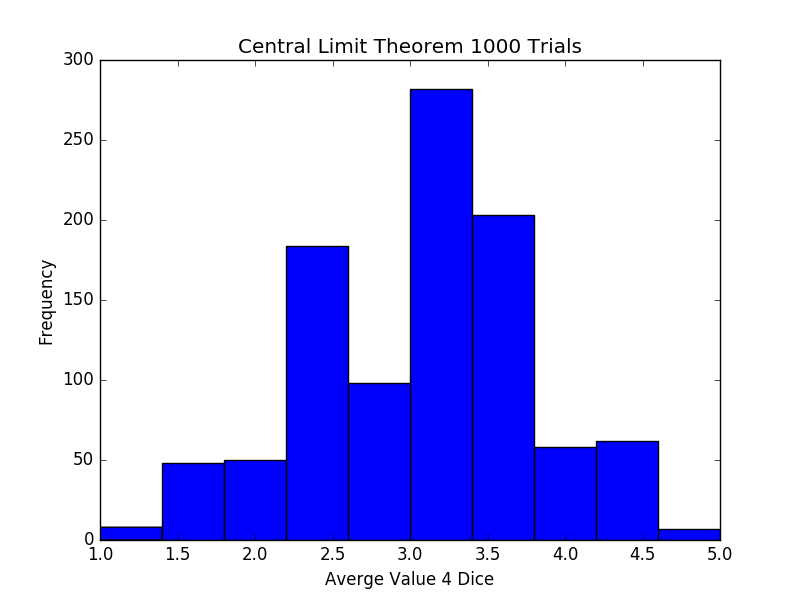
\includegraphics[scale=0.44]{clt1000.png}}
\subfigure[Individual Functions]{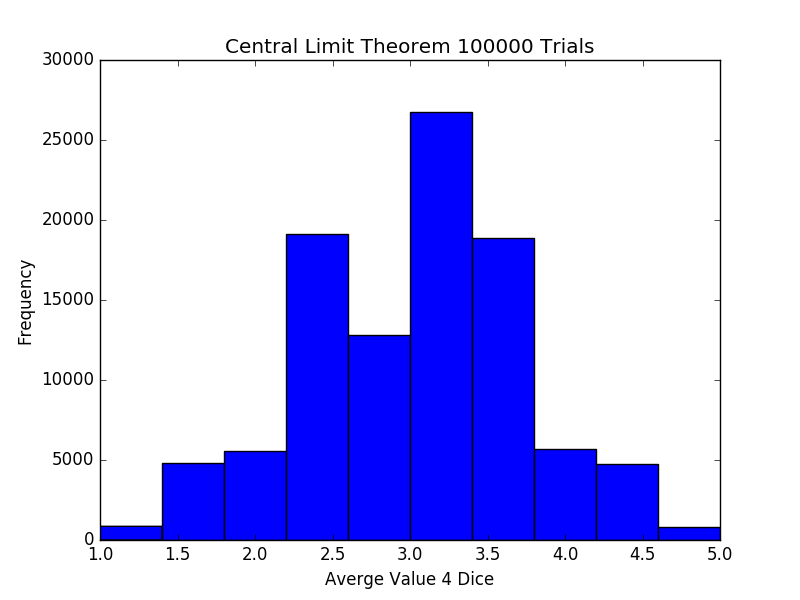
\includegraphics[scale=0.44]{clt100000.png}}
\subfigure[Integrand Scaling]{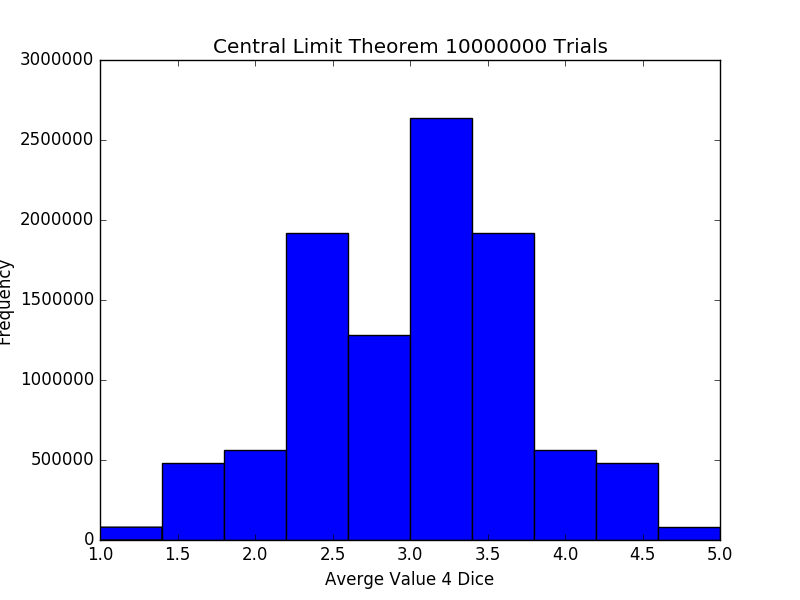
\includegraphics[scale=0.44]{clt10000000.png}}
\caption{Central Limit Theorem; As we make more measurements we better approximate a normal distribution.}
\end{figure}
A side comment, these plots do not look amazingly more Gaussian with more numbers. 
This is actually a programming problem, it is very difficult to generate random numbers in a computer.
The result that all of these trials have the dip between 2.5-3 is an artifact of 'bias' in the random number generator used in Python. 

\end{document}